%\documentclass[english,10pt]{beamer}
\documentclass[english,  handout]{beamer}






 
%\usepackage{mathptmx}
%\renewcommand{\sfdefault}{lmss}
\usepackage[T1]{fontenc}
%\usepackage[latin9]{inputenc}
\usepackage[utf8]{inputenc}

\synctex=-1

\usefonttheme{professionalfonts}

%\setbeamertemplate{navigation symbols}{}
%\setbeamertemplate{caption}[numbered]


\useinnertheme{rectangles}
%http://tex.stackexchange.com/questions/11168/change-bullet-style-formatting-in-beamer

 \AtBeginDocument{
  \addtolength\abovedisplayskip{-0.4\baselineskip}%
  \addtolength\belowdisplayskip{-0.4\baselineskip}%
}%change the space between text lines and the math formula


\usepackage{pifont}
%Postscript ZipfDingbats font
%the command \ding{number}, will print the specified symbol

\usepackage{fontawesome}
%icon package
\DeclareFontFamily{U}{FontAwesomeOne}{}
\DeclareFontShape{U}{FontAwesomeOne}{m}{n}{<-> FontAwesome--fontawesomeone}{}
\DeclareRobustCommand\FAone{\fontencoding{U}\fontfamily{FontAwesomeOne}\fontseries{m}\fontshape{n}\selectfont}
\DeclareFontFamily{U}{FontAwesomeTwo}{}
\DeclareFontShape{U}{FontAwesomeTwo}{m}{n}{<-> FontAwesome--fontawesometwo}{}
\DeclareRobustCommand\FAtwo{\fontencoding{U}\fontfamily{FontAwesomeTwo}\fontseries{m}\fontshape{n}\selectfont}
\DeclareFontFamily{U}{FontAwesomeThree}{}
\DeclareFontShape{U}{FontAwesomeThree}{m}{n}{<-> FontAwesome--fontawesomethree}{}
\DeclareRobustCommand\FAthree{\fontencoding{U}\fontfamily{FontAwesomeThree}\fontseries{m}\fontshape{n}\selectfont}

%ftp://ftp.dante.de/tex-archive/fonts/fontawesome/doc/fontawesome.pdf
%http://tug.ctan.org/info/symbols/comprehensive/symbols-a4.pdf


\usepackage{amsmath,amssymb,amsfonts,bm,mathrsfs,mathtools}

\usepackage{tikzsymbols}
%\usepackage[tikz]{bclogo}



\usepackage{perpage}
\MakePerPage{footnote} %reset for each page
%\renewcommand{\thefootnote}{\fnsymbol{footnote}} %use symbol, limit less than 9 symbols



%%%% HIGHTLIGHT  and annotation &=%%%%%%%%
\usepackage{color,xcolor}
 \usepackage{todonotes}

\usepackage[normalem]{ulem}

\usepackage[many]{tcolorbox}

\tcbset{fonttitle=\scriptsize}
\tcbset{highlight math style={enhanced,
  colframe=red!40!black,colback=yellow!20!white,arc=2pt,boxrule=.2pt,
  }}
  \newtcbox{\otherbox}[1][]{nobeforeafter,math upper,tcbox raise base,
enhanced,frame hidden,boxrule=0pt,interior style={top color=green!10!white,
bottom color=green!10!white,middle color=green!50!yellow},
fuzzy halo=1pt with green,#1}
%%\tcbhighmath{math here}
%% \otherbox{math here}



%%%%% HIGHLIGHT %%%%%%
\newcommand{\hb}[1]{{\color{blue}{#1}}}
%\noindent\rule{\textwidth}{.5pt}

%:
\usepackage{soul}

\newcommand\hcancel[2][black]{\setbox0=\hbox{$#2$}%
\rlap{\raisebox{.45\ht0}{\textcolor{#1}{\rule{\wd0}{1pt}}}}#2}
%cross to delete

\newcommand{\mcb}[2]{\colorbox{#1}{$\displaystyle #2$}}
%highlight math

\newcommand{\hlfancy}[2]{\sethlcolor{#1}\hl{#2}}
%specified color , for\hl

\newcommand\myhl{\bgroup\markoverwith
  {\textcolor{yellow}{\rule[-.5ex]{2pt}{2.5ex}}}\ULon}



\mode<presentation>{ \usetheme{boxes} }

%write Matlab code
\usepackage{listings}
 \definecolor{dkgreen}{rgb}{0,0.6,0}
\definecolor{gray}{rgb}{0.5,0.5,0.5}
\definecolor{mauve}{rgb}{0.58,0,0.82}
\lstset{frame=tb,
  language=Matlab,
  aboveskip=3mm,
  belowskip=3mm,
  showstringspaces=false,
  columns=flexible,
  basicstyle={\small\ttfamily},
  numbers=none,
  numberstyle=\tiny\color{gray},
  keywordstyle=\color{blue},
  commentstyle=\color{dkgreen},
  stringstyle=\color{mauve},
  breaklines=true,
  breakatwhitespace=true
  tabsize=3
}

\usepackage[lastexercise]{exercise}

\newtheorem{ex}{Exercise}
\newtheorem{property}{Property}
\newtheorem{ag}{Algorithm}
\newtheorem{remark}{Remark}
\newtheorem{den}{definition}
\newtheorem{assumption}{Assumption}


\usepackage[nosolutionfiles]{answers}
\Newassociation{sol}{Solution}{ans}



\usepackage{empheq}
\usepackage{comment}
%\usepackage{lscape}
\usepackage{multirow}
\usepackage{url,hyperref}

\hypersetup{
 %   bookmarks=true,         % show bookmarks bar?
    unicode=false,          % non-Latin characters in Acrobat's bookmarks
    pdftoolbar=true,        % show Acrobat's toolbar?
    pdfmenubar=true,        % show Acrobat's menu?
    pdffitwindow=false,     % window fit to page when opened
    pdfstartview={FitH},    % fits the width of the page to the window
    pdftitle={My title},    % title
    pdfauthor={Author},     % author
    pdfsubject={Subject},   % subject of the document
    pdfcreator={Creator},   % creator of the document
    pdfproducer={Producer}, % producer of the document
    pdfkeywords={keyword1} {key2} {key3}, % list of keywords
    pdfnewwindow=true,      % links in new window
    colorlinks=true,       % false: boxed links; true: colored links
    linkcolor=red,          % color of internal links (change box color with linkbordercolor)
    citecolor=green,        % color of links to bibliography
    filecolor=magenta,      % color of file links
    urlcolor=cyan           % color of external links
}


\usepackage{subfigure,epsfig,graphicx,graphics}

\DeclareGraphicsRule{.tif}{png}{.png}{`convert #1 `dirname #1`/`basename #1 .tif`.png}
   \DeclareGraphicsExtensions{.pdf}




\newcommand{\hw}{ {\underline{\tt Homework }} }
\newcommand{\hws}{ {\underline{\tt Homework$\star$}} }
\newcommand{\optional}{ {\it optional} }

\newcommand{\MATLAB}{ \texttt{MATLAB}}
\newcommand{\python}{ \texttt{python}}
\newcommand{\Rlang}{ \texttt{R}}
\newcommand{\SAS}{ \texttt{SAS}}
\newcommand{\MC}{Markov Chain}


\newcommand{\tm}{transition matrix}
\newcommand{\rv}{random variable}
\newcommand{\spl} {supervised learning }
 

\newcommand{\dis}{\underline{\tt discussion}: }
\newcommand{\pri}{\underline{\tt principle}: }




\newcommand{\bq}{\scalebox{6}{\textbf{?} }}
\newcommand{\sq}{\scalebox{2}{\textbf{?} }}
\newcommand{\ck} {  {\scalebox{0.8} {\Interval}   } }

\newcommand{\eps}{\varepsilon}
\newcommand{\To}{\longrightarrow}

% 
\newcommand{\Dcal}{\mathtt{D}}
\newcommand{\Hcal}{\mathcal{H}}
\newcommand{\Ecal}{\mathcal{E}}
\newcommand{\Xcal}{\mathcal{X}}
\newcommand{\Ycal}{\mathcal{Y}}
\newcommand{\Zcal}{\mathcal{Z}}

%%Calculus 

\renewcommand{\d}{\ensuremath{\mathrm{d}}}
\newcommand{\dt}{ \ensuremath{\mathrm{d} t } }
\newcommand{\dx}{ \ensuremath{\mathrm{d} x} }
\newcommand{\dy}{ \ensuremath{\mathrm{d} y } }

%indicator function
\newcommand{\indf}{ \ensuremath{\mathbf{1} } }



%probability
\newcommand{\p}{ \mathbb{P}}
\newcommand{\prob}{{\Pr}}
\newcommand{\PP}{\mbox{PP}}%Poisson process
%condition prob
\newcommand{\cPr}[2]{{\Pr\left(#1\mid #2\right)}}

\newcommand{\FF}{{\mathbb{F}}}

\newcommand{\e}{ \operatorname{\mathbb E}}
\newcommand{\Var}{\operatorname{\mathbb{V} }}
\newcommand{\var}{\operatorname{\text{Var} }}
\newcommand{\MSE}{\operatorname{\text{MSE} }}

\newcommand{\Std}{\operatorname{std}}
\newcommand{\Cov}{\operatorname{cov}}

%Matrix  %mathbf
\newcommand{\Pb}{{\mathbf{P}}}
\newcommand{\Qb}{{\mathbf{Q}}}
\newcommand{\Mb}{{\mathbf{M}}}
\newcommand{\cb}{\mathbf{c}}
\newcommand{\bb}{{\mathbf{b}}}

\newcommand{\Tb}{\mathbf{T}}

\newcommand{\Wb}{\mathbf{W}}
\newcommand{\wb}{\mathbf{w}}
\newcommand{\Xb}{\mathbf{X}}

\newcommand{\xb}{\mathbf{x}}

\newcommand{\Wtn}{\mathbb{W}}
\newcommand{\btn}{\mathbf{b}}



\newcommand{\eye}{{\mathbf{I}}}
%identity matrix
\newcommand{\onem}{{\mathbb{1}}}
\newcommand{\idor}{\mathbf{1}}
\newcommand{\ii}{\mathbf{i}}
%imaginary symbol

\usepackage{tikz}

%State number
\newcommand{\snum}[1]{ \raisebox{.5pt}{\textcircled{\raisebox{-.9pt} {#1}}}}

 \usetikzlibrary{arrows}
\usetikzlibrary{shapes}

%\newcommand{\snum}[1]{%
 % \tikz[baseline=(char.base)]\node[anchor=south west, draw,rectangle, rounded corners, inner sep=1.4pt, minimum size=5mm,
   % text height=1.3mm](char){\ensuremath{#1}} ;}

\newcommand*\circled[1]{\tikz[baseline=(char.base)]{
            \node[shape=circle,draw,inner sep=.4pt] (char) {#1};}}


%real number
\newcommand{\Real}{{\mathbb{R}}}
%integer
\newcommand{\ZZ}{\mathbb{Z}}
%positive integer
\newcommand{\NN}{\mathbb{N}}



\newcommand{\inpd}[2]{\left\langle #1, #2 \right\rangle}
\newcommand{\abs}[1]{\left\vert#1\right\vert}
\newcommand{\norm}[1]{\left\|#1\right\|}
\newcommand{\wt}[1]{{\widetilde{#1}}}
\newcommand{\set}[1]{\left\{#1\right\}}
\newcommand{\partiald}[2]{  \frac{\partial #1 }{\partial #2}}



\newcommand{\ie}{{\it{i.e.}}}



\newcommand{\transpose}{\textsf{T}} % or, \intercal
\newcommand{\diag}{\textsf{diag}}
\newcommand{\tr}{{\textsf{T}}}
\newcommand{\rt}{{\textbf{r}}}

\DeclareMathOperator{\trace}{Trace}


\newcommand{\argmin}{ \operatornamewithlimits{argmin} }
\newcommand{\argmax}{ \operatornamewithlimits{argmax} }




\def\biz{\begin{itemize} }
\def\bizp{\begin{itemize}[<+->] }
\def\eiz{\end{itemize}}


\def\bfm{\begin{frame}}
\def\efm{\end{frame}}

\def\bena{\begin{enumerate}[<+-| alert@+>]}
\def\ben{\begin{enumerate}}
\def\een{\end{enumerate}}


\def\bbk{\begin{block} }
\def\ebk{\end{block}}






\makeatletter
%%%%%%%%%%%%%%%%%%%%%%%%%%%%%% Textclass specific LaTeX commands.
 % this default might be overridden by plain title style

%%%%%%%%%%%%%%%%%%%%%%%%%%%%%% User specified LaTeX commands.
%\usetheme{Warsaw}
\usetheme{Boadilla}
% or ...



%\setbeamertemplate{footline}[text line]{} % makes the footer EMPTY
%\setbeamertemplate{footline}[page number]{} % makes the footer EMPTY

%\usecolortheme{orchid} %not use is better 

\setbeamertemplate{footline}[text line]{%
  \parbox{\linewidth}{\vspace*{-2pt}Xiang Zhou\hfill CityU\hfill \insertpagenumber}}
%\setbeamertemplate{navigation symbols}{}

%\setbeamercovered{transparent}
% or whatever (possibly just delete it)


%\usepackage{babel}
\makeatother



 %
%\addtobeamertemplate{frametitle}{}{%
%\begin{tikzpicture}[remember picture,overlay]
%\node[anchor=south east,yshift=2pt] at (current page.south east) {
\includegraphics[height=0.6cm]{CityU_Logo_Basic_Signature.eps}};
%\end{tikzpicture}}
%

\beamerdefaultoverlayspecification{<+->}
%the presentation acts as though a \pause command has been inserted between every two bullets, without the actual need to write \pause after each item.



\title{Classification: Support Vector Classifier}
\author{
\includegraphics[height=1.1cm,width=2.2cm]{../CityU_Logo_Basic_Signature.eps}
\\ $\ $ \\
Xiang Zhou  \\ $\ $ \\
}
\institute[]{  School of Data Science 
\\
 Department of Mathematics
\\
City University of Hong Kong
\\
~~
\\
\textup{  }
}

\date[]{}



\begin{document}
 
 


\maketitle
 
 
 
\frame{{SVM}
developed by computer science 

\biz
\item Vapnik 1995:  Geometric Viewpoint + Primal-Dual for Quadratic Programming (+ Kernel trick, new def of metric)   ~~
\item Sollich 2002: \href
{https://link.springer.com/content/pdf/10.1023/A:1012489924661.pdf}{Bayesian Viewpoint} 
\eiz

\begin{table}
\begin{center}
\begin{tabular}{c|c}
Method & main properties
\\
\hline
\hline
{maximal margin classifier}
 & only for linear separable dataset
  \\
\hline
  {support vector classifier}
  & slack variable, linear classifier 
 \\
 \hline
  {support vector machine} & kernel trick, nonlinear classifier
  \\ \hline
\end{tabular}
\end{center}
\caption{Development of SVM}
\end{table}
\footnote
{
We do not  discuss here the numerical optimization   part of SVM 
(a good example for convex optimization .
online resource: \url{http:/uito/www.robots.ox.ac.uk/~az/lectures/ml/index.html}).
The focus here is the geometric intuition and modelling.
}

}
\frame{{Linear Separable Problem}
Binary classification problem:  dataset $\set{x_i, y_i}$ where $y_i\in \mathcal{Y}=\set{-1,1}$.
Recall 
\biz
\item Logistic regression assumes: log odd $\log h(x)$ is linear in $x$. 
The decision boudary
$h(x)=0.5$ is equivalent to $\beta \cdot x   =0.5$ 
\item The LDA's  the discriminant function $\delta(x)$ is also linear in $x$.
\item SVM is also a linear classifier, with a strong geometric intuition.
\eiz


 \begin{remark}
 \biz
 \item 
The logistic  regression =
sigmoid  activation function 
+ 
linear feature assumption 
+ maximum likelihood
\item 
The  linear discriminant analysis (LDA) =
Bayes classifier +  Gaussian mixture +
equal variance   assumption  
\item 
The support vector machine (SVM) = 
linear classifier 
+ max margin
\eiz
\end{remark}

}

\frame{Note the notations different from logistic regressions:
\biz
\item $\mathcal{Y} =\set{-1,1}$, not $\set{0,1}$
\item the discriminant function is generally denoted by $f$.
The classifier  $\phi(x) := \mbox{sign} f(x)\in \set{-1,1}$.
Then decision boundary is $f(x)=0$, not $h(x)=0.5$.
\eiz
This set of notation is convenient because
if $y $ belong to $ \set{-1,1}$
$$\otherbox
{\mbox{sign} f(x) = y \iff  y f(x)  >0.}$$ 

 Remember $\mbox{sign} f(x)  = \mbox{sign}( \lambda f(x) )$ for any $\lambda>0$. 

{\rule{\paperwidth}{0.5pt}}
The 0-1 loss then can be written as
$$
\ell_{01}(f(x), y) =   1- \mbox{heaviside}(y f(x) ) 
= (1-\mbox{sign}(y f(x) ))/2 $$
which is equal to 
$\ell_{01}(\phi(x),y)=
\ell_{01}(\mbox{sign}f(x), y)$.
We extend $\ell_{01}$'s  domain $\Ycal\times \Ycal$
to $\Real\times \Real$.

}

\frame{

\begin{ex}
 A linear discriminant function is $f(x)=w\cdot x + b$.
Only the sign matters, so w.l.o.g., we assume $\norm{w}=1$.
Given a point $x^*$, show the  signed distance between $x^*$
and the hyperplane $f(x)=0$ is $$ {f(x^*)}$$ ( or $f(x^*)/\norm{w}$ in general).
\end{ex}
}

\frame{
Given one data example $(x_i, y_i)$,
if $f$ correctly classifies $x_i$, then $\mbox{sign} f(x_i)=y_i$
the  distance to the hyperplane $f(x)=0$ is 
$$\abs{f(x_i)} = f(x_i) \cdot \mbox{sign} f(x_i) = \tcbhighmath{f(x_i) y_i }=:M_i,$$
which is   the {\bf  margin} from $x_i$ to the separating hyperplane.
 
\begin{den}[margin]
Given   the dataset $(x_i, y_i), i=1,\ldots, n$  
and a linear function $f(x)=w\cdot x+b$, then 
the margin of the dataset $(x_i, y_i), i=1,\ldots, n$ to the hyperplane $f(x)=0$ is 
\[
M= \min_{1\leq i \leq n}  \set{ y_i (w\cdot x_i +b) / \norm{w} }
\]
The support vectors are the collection of $\set{x_j}$
such that $M=y_j (w\cdot x_j +b)$.
Sometimes, the margin refers to the two hyperplanes 
$w\cdot x + b = \pm M/\norm{w}$ where support vectors lie.
\end{den}
$M>0 \iff $ the dataset is linearly separable, i.e. 
$$\mbox{sign}f(x_i) = y_i, \forall i.$$
}

\frame{
\begin{definition}[maximal margin classifier]
{The maximal margin classifier} solves the problem 
\begin{equation}\label{eq:mmc}
\begin{split}
&\max_{w\in \Real^d,b\in \Real} M
\\
\mbox{subject to} ~&~~
\norm{ w} =1\\
&  y_i (w\cdot x_i +b) \geq M , \forall i
\end{split}
\end{equation}
\end{definition}
\biz
\item 
The equivalent form of maximal margin classifier is
\begin{equation}\label{eq:mmc2}
\begin{split}
&\max_{w\in \Real^d,b\in \Real} M
\\
\mbox{subject to} ~~
 &  y_i (w\cdot x_i +b) / \norm{w}\geq M , ~~\forall i
\end{split}\end{equation}
\item The constraint $\norm{w}=1$ is only for the uniqueness of $w$ and $b$;
without this constraint, the solution  is a family of the linear discriminant functions
$\set{\lambda f^{*}(x): \lambda>0}$, which all share 
the {\bf same} classifier $\phi^{*}=\mbox{sign}f$.

\item This form is applicable to non linear separable case.
If the maximal $M$ is negative, then the dataset is not linearly separable. 
Otherwise, the dataset is   linearly separable.
\eiz

}

\frame{
\begin{ex}[XOR]
Suppose the dataset has $n=4$ examples as follows:
\begin{tabular}{ll}
$ x_1$=(1, -1)&  $y_1$ = -1\\
 $x_2$=(1, 1) &  $y_2$ =   1\\
 $x_3$=(-1, 1)&  $y_3$ = -1\\
 $x_4$=(-1, -1)&  $y_4$ = 1
\end{tabular}.
Find the maximal margin classifier $f(x)=w_1 x_{(1)} + w_2 x_{(2)} + b$.
\end{ex}
{\footnotesize
\begin{align*}
&\max_{w\in \Real^d,b\in \Real} M
\\
\mbox{subject to} ~&~~
w_1^2 + w_2^2 =1\\
&  w_1 + w_2 + b \geq M  
\\
&  -w_1 - w_2 + b \geq M  
\\&
  w_1 - w_2 - b \geq M  
  \\&
    -w_1 + w_2 - b \geq M  
\end{align*} 
The constraints are equivalent to $\abs{w_1+w_2}\leq -M+b$ and $\abs{w_1-w_2}\leq -M-b$.
Then $\abs{w_1}\leq -M$. So any admissible $M$ is negative.
It is easy to show that 
$M\pm b\leq 0$. So the possible max of $M$ is $M=b$ or $M=-b$.
If $M=b$, then $w_1=-w_2=\pm b$ and $f(x)=(-x_1+x_2\pm1)/\sqrt{2}$.
If $M=-b$, then $w_1=w_2=\pm b$ and the solution is 
$f(x)=(-x_1-x_2\pm1)/\sqrt{2}$
}

}


\frame{
The alternative form of maximal margin classifier is
\begin{align*}
&\max_{w\in \Real^d,b\in \Real} M
\\
\mbox{subject to} ~~
 &  y_i (w\cdot x_i +b) / \norm{w}\geq M , ~~\forall i
\end{align*}
Since we can scale $w,b$ by a {\bf positive} factor arbitrarily, we
can assume  $M>0$ and $ M \norm{w} =1 $ {\it if the dataset is linearly separable},
instead of using the rescaling $\norm{w}=1$.
Then
\begin{equation}\label{eq:mmc3}
\begin{split}
&\min_{w\in \Real^d,b\in \Real} \frac12 \norm{w}^2
\\
\mbox{subject to} ~~
 & \tcbhighmath{ y_i (w\cdot x_i +b) \geq 1 , \forall i}
\end{split}
\end{equation}
\biz
\item
Now there is NO solution if not linear separable, in contrast to  \eqref{eq:mmc2} and \eqref{eq:mmc}.
\item The problem  \eqref{eq:mmc3} is the standard quadratic programming problem \faSmileO ,
in contrast to  \eqref{eq:mmc2} and \eqref{eq:mmc}.
\item
The margin corresponds to the equalities when the inequality constraint, i.e., 
the  two parallel hyperplanes for the margin are given 
\[ \boxed{ w\cdot x + b =\pm 1}.\]
The margin width is $\frac{2}{\norm{w}}$
\par 
\eiz

}


\frame{{Support Vector Classifier}
\framesubtitle
{soft margin and slack variable}

\underline{But linear separation assumption is too strong in practice}

The non-separable case means there are some examples $(x_m, y_m)$ such that
$y_m (w\cdot x_m +b) < 0$.  Then by adding $n$ slack variables $\xi=(\xi_1,\ldots, \xi_n)$, we have the support vector classifier 
\begin{definition}[support vector classifier]
\begin{align}
&\min_{w\in \Real^d,b\in \Real} \frac12 \norm{w}^2
\\
\mbox{subject to} ~~
 &  y_i (w\cdot x_i +b) \geq 1-\xi_i , \forall i
 \\
 &\xi_i \geq 0, \forall i
 \\
 & \sum_{i=1}^n {\xi_i} \leq const
\end{align}
where $const>0$ is a tuning parameter.
\end{definition}
$const=0\iff$ maximal margin classifier (for linear separable case), do not allow violation of the margin.
\par
If $const=\infty$, then  $w=0$, $b$ arbitrary. No data $(x_i, y_i)$ is used.
}
\frame{{Understand SVC's geometric perspective}
\biz
\item The margin is given by two hyperplanes :  $w\cdot x + b= \pm 1$
with the margin gap $2M=\frac{2}{\norm{w}}$.
\item $\xi_i >1$ means  $y_i (w\cdot x_i +b)$ is negative:      $y_i$ is on the other side of the hyperplane predicted by $f(x)$ .
\item $\xi_i >0$ then $y_i$ violates the margin;
\item $\xi_i = 0$, then $y_i$ is on the same side predicted by the margin;
Furthermore,  $y_i (w\cdot x_i +b)  = 1 \iff $ support vectors  
\eiz

}


\frame{
Note that $ y_i f(  x_i  ) \geq 1-\xi_i  $  and $\xi_i \geq 0$ together 
are equivalent to $\xi_i \geq \max\set{0, 1-y_if(x_i)}=: (1-y_i f(x_i))_+$.
Then the SVC 
\begin{align*}
&\min_{w\in \Real^d,b\in \Real} \frac12 \norm{w}^2
\\
\mbox{subject to} ~~
  &\xi_i \geq (1-y_i (w\cdot x_i + b))_+, \forall i
 \\
 & \sum_{i=1}^n {\xi_i} \leq const
\end{align*}
is equivalent to 
\begin{align*}
&\min_{w\in \Real^d,b\in \Real} \frac{1}{2C} \norm{w}^2 + \sum_{i} \xi_i
\\
\mbox{subject to} ~~
  &\xi_i \geq (1-y_i (w\cdot x_i + b))_+, \forall i
 \end{align*}
 which is equivalent to
 \begin{equation}
\min_{w\in \Real^d,b\in \Real} \frac{1}{2C} \norm{w}^2 + \sum_{i} (1-y_i (w\cdot x_i + b))_+
 \end{equation}
 This is the form of  (hinge) loss + ($L_2$) regularization
 

}
\frame{
{\bf SVC :  hinge Loss + Regularization}
\begin{equation}
\min_{w,b} \sum_{i=1}^n  \ell_{\mbox{hinge}}(y_i, f(x_i)) + \frac{C}{2}\norm{w}^2
\end{equation}

where $f(x)=w\cdot x +b$ and 
\[
\otherbox{
\ell_{\mbox{hinge}}(y,f) = (1-y f)_+ , ~~ y\in \set{-1,1}, f \in \Real}
\]
$C=\infty\iff w=0$; \par$C=0\Longrightarrow$  (1) min=0 means the linear separation case
(2) min $>0$ is the non separable; in both, the solution $f^*$ is not unique, even restricted to linear. 
}

\frame{
 {\bf logistic regression :  binomial deviance Loss without  Regularization}

Recall the logistic regression solves
\begin{equation}
\min_{f}  \e \ell_{\mbox{bd}}(Y, f(X))  \approx  \frac{1}{n} \sum_{i=1}^n  \ell_{\mbox{bd}}(y_i, f(x_i)) 
\end{equation}
where $f(x)=\mbox{logit}(h)=\log \frac{h}{1-h}$ with $h(x)=\p(Y=+1\vert X=x)$
and the binomial deviance loss
\[
\ell_{\mbox{bd}}(y,f)=\log (1+e^{-yf}), ~~y\in \set{-1,1}.
\]
}
\frame{
Recall the 0-1 loss \eqref{01loss} in the Bayesian classifier, we rewrite it in term of $f$: 
$\ell_{01}(y,f) 
 =\idor(y \neq \mbox{sign}(f(x)) )= \begin{cases}
1 & \mbox{if }  y  f(x)<0  \\
0   & \mbox{if }  yf(x)>0  
\end{cases}=1- \mbox{Heaviside}(yf)$.
Then we have three loss functions $\ell_{\mbox{bd}}$, $\ell_{\mbox{hinge}}$, $\ell_{01}$
which are all functions effectively in term of the product $yf(x)$
\begin{figure}[htbp]
\begin{center}
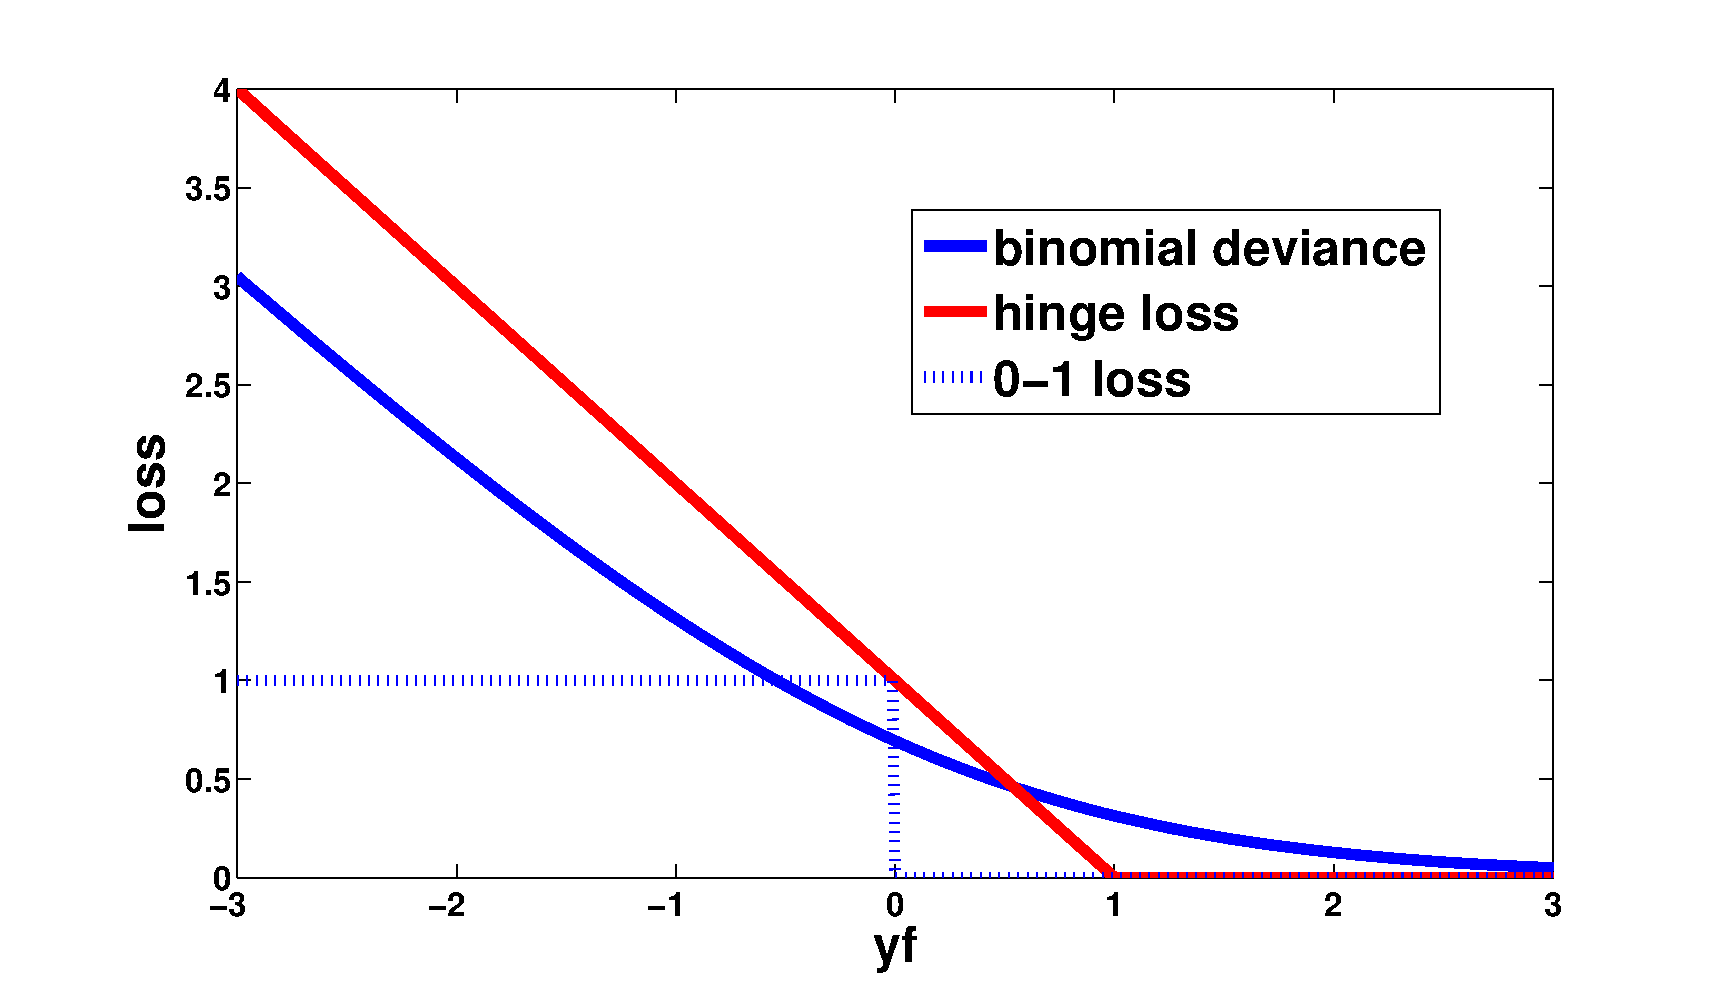
\includegraphics[width=0.6\textwidth]{lossclassification.eps}
  \end{center}
\end{figure}
\dis { What differences ?  Computational issues ? Which data examples
feel the ``gradient'' force?
Why need regularization for hinge?
What else of loss function do you like to propose ? }

}

\frame{

We already know that the optimal solution to the 0-1 loss 
\[ \inf_f \e \ell_{0,1} (Y, f(X))\]
is Bayesian classifier $\phi^*(x)=\mbox{sign}(f^*) =\mbox{sign} ( h(x) - 0.5)$
where $h(x)=\p(Y=+1\vert X=x)$. Only the sign $f^*$ is determined.

\begin{ex}
Consider the minimization problem 
\[ \inf_f \e \ell_{\mbox{bd}} (Y, f(X))\]
for the $\set{\pm 1}$-encoded binary classification problem.
Show that the optimal $f^*$ is the log odd:
 $$f^*(x)=\mbox{logit}(h(x))=\log \frac{h}{1-h}$$ where $h(x)=\p(Y=+1\vert X=x)$.
\end{ex}
The two problems are not variation of calculus, but are solved in point-wise sense.
}

\frame{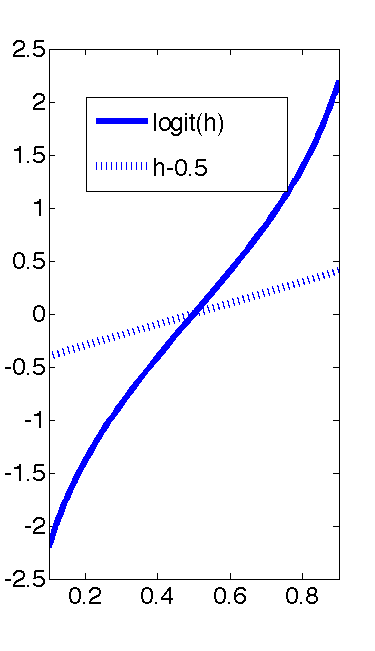
\includegraphics[width=0.3\textwidth]{logith.png}}
\frame{Kernel logistic regression vs Kernel SVM
\url{https://stats.stackexchange.com/questions/43996/kernel-logistic-regression-vs-svm}
}
\include{svmtalk.pdf}

\end{document}


